% !Mode:: "TeX:UTF-8" 



\BiSection{2.15}{Figures}

\fancyhead[R]{本题2.15由QC.Z完成}

		\begin{figure}[H] %H为当前位置,!htb为忽略美学标准,htbp为浮动图形
	\begin{minipage}{\linewidth}
		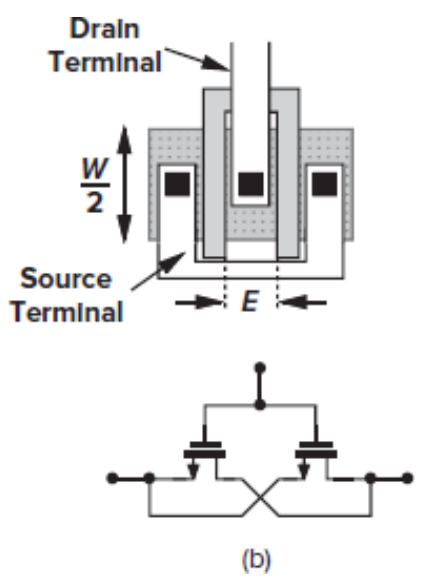
\includegraphics[width=1\linewidth]{2.33b-s}
	\end{minipage}
	\caption*{图2.33} %最终文档中希望显示的图片标题
\end{figure}

解:

图1展示教材图2.33(b)的基底连接

		\begin{figure}[H] %H为当前位置,!htb为忽略美学标准,htbp为浮动图形
	\begin{minipage}{\linewidth}
		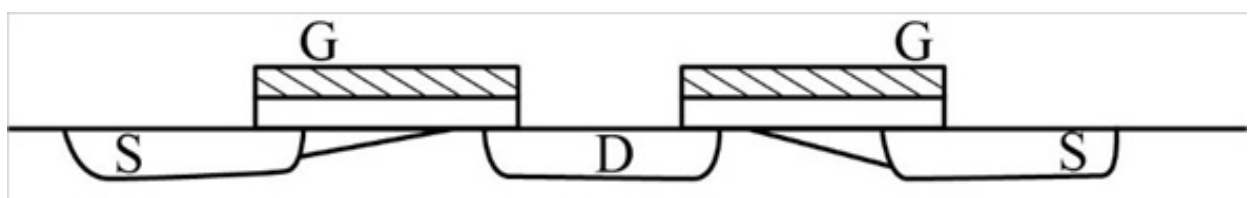
\includegraphics[width=1\linewidth]{2.15-1}
	\end{minipage}
	\caption*{图1} %最终文档中希望显示的图片标题
\end{figure}

因此每单位宽度$C_{GD}=2(\frac{W}{2}C_{ov})$

把每单位宽度重叠电容$C_{ov}\cong L_DC_{ox}$带入前式有

$C_{GD}=2(\frac{W}{2}L_DC_{ox})=WL_DC_{ox}$

\begin{figure}[H] %H为当前位置,!htb为忽略美学标准,htbp为浮动图形
	\begin{minipage}{\linewidth}
		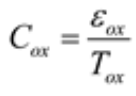
\includegraphics{2.15-2}
	\end{minipage}
\end{figure}


\begin{figure}[H] %H为当前位置,!htb为忽略美学标准,htbp为浮动图形
	\begin{minipage}{\linewidth}
		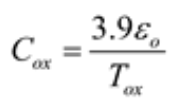
\includegraphics{2.15-3}
	\end{minipage}
\end{figure}


\begin{figure}[H] %H为当前位置,!htb为忽略美学标准,htbp为浮动图形
	\begin{minipage}{\linewidth}
		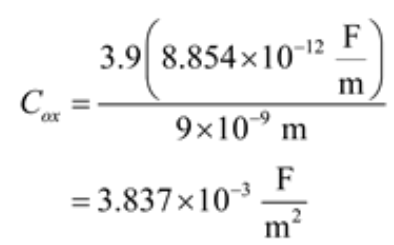
\includegraphics{2.15-4}
	\end{minipage}
\end{figure}

\begin{figure}[H] %H为当前位置,!htb为忽略美学标准,htbp为浮动图形
	\begin{minipage}{\linewidth}
		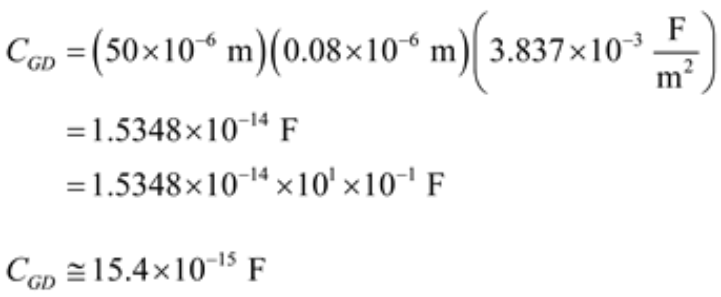
\includegraphics{2.15-5}
	\end{minipage}
\end{figure}


\begin{figure}[H] %H为当前位置,!htb为忽略美学标准,htbp为浮动图形
	\begin{minipage}{\linewidth}
		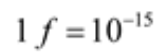
\includegraphics{2.15-6}
	\end{minipage}
\end{figure}


\begin{figure}[H] %H为当前位置,!htb为忽略美学标准,htbp为浮动图形
	\begin{minipage}{\linewidth}
		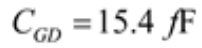
\includegraphics{2.15-7}
	\end{minipage}
\end{figure}

由教材图2.33(b)每单位宽度$C_{GS}=\frac{2WLC_{ox}}{3}+WC_{ov}=\frac{2WLC_{ox}}{3}+WL_DC_{ox}=WC_{ox}(\frac{2L}{3}+L_D)$

\begin{figure}[H] %H为当前位置,!htb为忽略美学标准,htbp为浮动图形
	\begin{minipage}{\linewidth}
		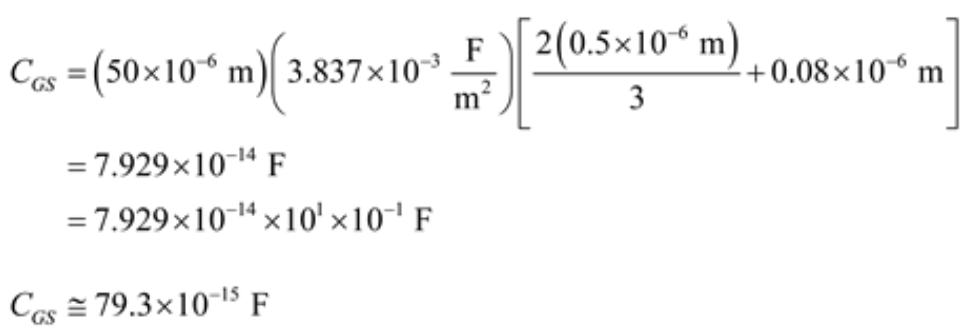
\includegraphics{2.15-8}
	\end{minipage}
\end{figure}


\begin{figure}[H] %H为当前位置,!htb为忽略美学标准,htbp为浮动图形
	\begin{minipage}{\linewidth}
		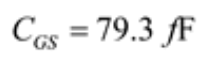
\includegraphics{2.15-9}
	\end{minipage}
\end{figure}


修改后的教材2.33(b)重画于图2


		\begin{figure}[H] %H为当前位置,!htb为忽略美学标准,htbp为浮动图形
	\begin{minipage}{\linewidth}
		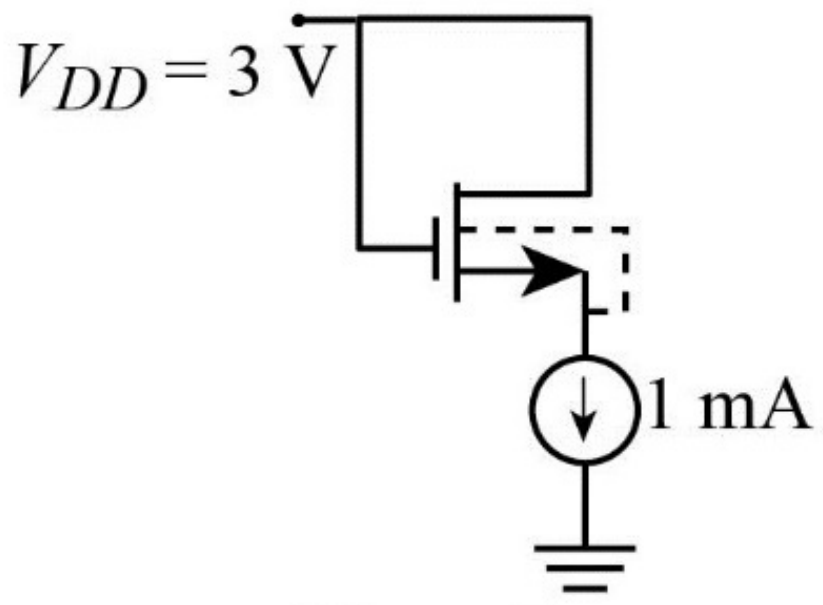
\includegraphics[width=1\linewidth]{2.15-10}
	\end{minipage}
	\caption*{图2} %最终文档中希望显示的图片标题
\end{figure}



\begin{figure}[H] %H为当前位置,!htb为忽略美学标准,htbp为浮动图形
	\begin{minipage}{\linewidth}
		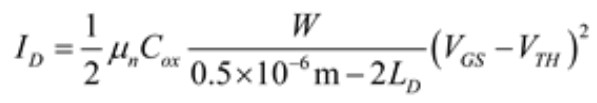
\includegraphics{2.15-11}
	\end{minipage}
\end{figure}

\begin{figure}[H] %H为当前位置,!htb为忽略美学标准,htbp为浮动图形
	\begin{minipage}{\linewidth}
		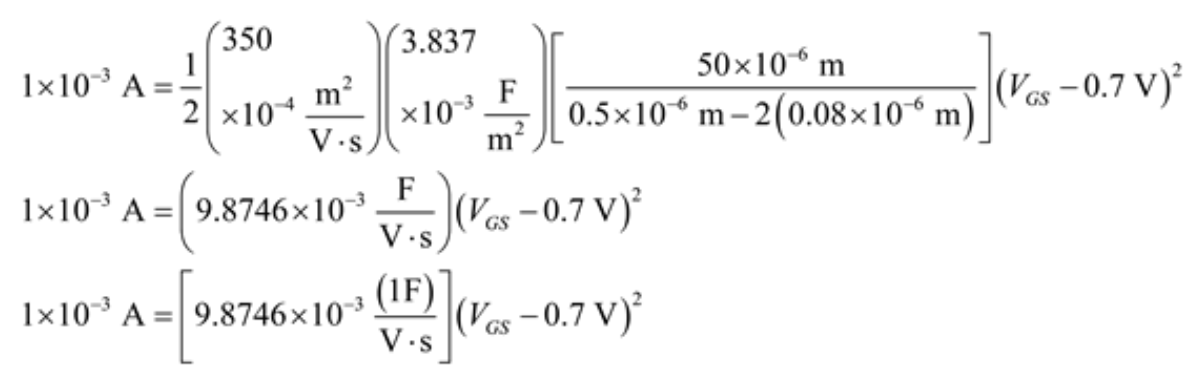
\includegraphics[width=1\linewidth]{2.15-12}
	\end{minipage}
\end{figure}


\begin{figure}[H] %H为当前位置,!htb为忽略美学标准,htbp为浮动图形
	\begin{minipage}{\linewidth}
		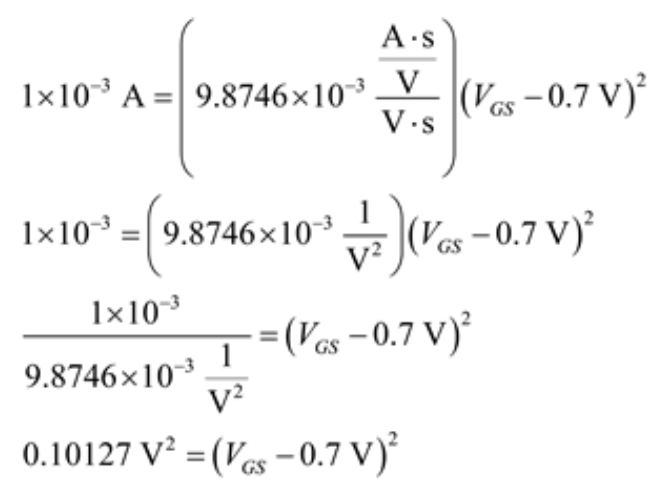
\includegraphics{2.15-13}
	\end{minipage}
\end{figure}


\begin{figure}[H] %H为当前位置,!htb为忽略美学标准,htbp为浮动图形
	\begin{minipage}{\linewidth}
		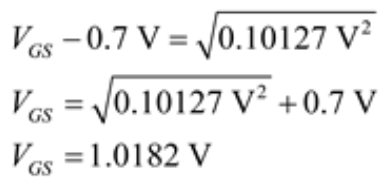
\includegraphics{2.15-14}
	\end{minipage}
\end{figure}

因为$V_{GS}=V_{DB}$所以$V_{DB}=1.0182V$

由教材图2.33(b)漏结电容$C_{DB}=\frac{W}{2}EC_j+2(\frac{W}{2}+E)C_{jsw}$其中$C_j$是每单位区域源漏下极板结电容,$C_{jsw}$是每单位长度源漏侧壁结电容,$E$是S/D区(横向)尺寸

\begin{figure}[H] %H为当前位置,!htb为忽略美学标准,htbp为浮动图形
	\begin{minipage}{\linewidth}
		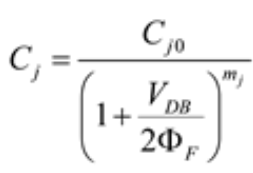
\includegraphics{2.15-15}
	\end{minipage}
\end{figure}

\begin{figure}[H] %H为当前位置,!htb为忽略美学标准,htbp为浮动图形
	\begin{minipage}{\linewidth}
		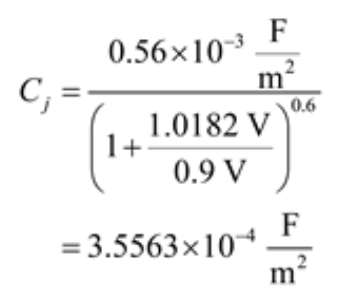
\includegraphics{2.15-16}
	\end{minipage}
\end{figure}


\begin{figure}[H] %H为当前位置,!htb为忽略美学标准,htbp为浮动图形
	\begin{minipage}{\linewidth}
		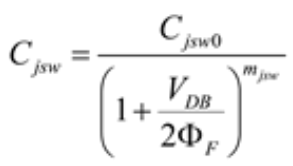
\includegraphics{2.15-17}
	\end{minipage}
\end{figure}


\begin{figure}[H] %H为当前位置,!htb为忽略美学标准,htbp为浮动图形
	\begin{minipage}{\linewidth}
		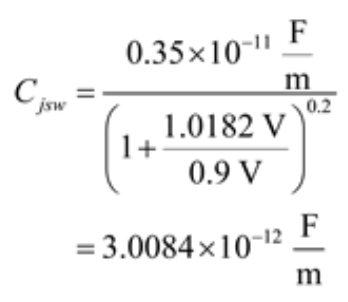
\includegraphics{2.15-18}
	\end{minipage}
\end{figure}

\begin{figure}[H] %H为当前位置,!htb为忽略美学标准,htbp为浮动图形
	\begin{minipage}{\linewidth}
		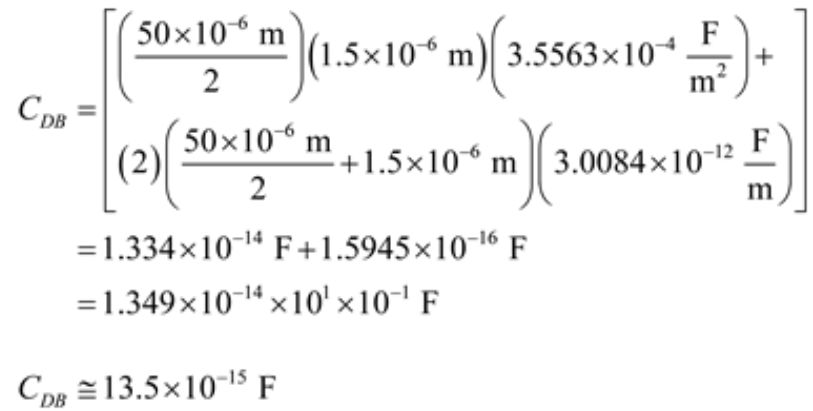
\includegraphics{2.15-19}
	\end{minipage}
\end{figure}

$C_{DB}=13.5fF$

由教材图2.33(b)源结电容$C_{SB}=2[\frac{W}{2}EC_j'+2(\frac{W}{2}+E)C_{jsw}']$

因为$C_j=C_j'$和$C_{jsw}=C_{jsw}'$

所以$C_{SB}=2C_{DB}=27fF$




由教材图2.33(b)栅结电容$C_{GB}=\frac{(WLC_{ox})C_d}{WLC_{ox}+C_d}$


\begin{figure}[H] %H为当前位置,!htb为忽略美学标准,htbp为浮动图形
	\begin{minipage}{\linewidth}
		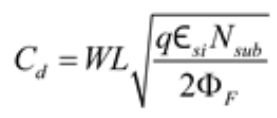
\includegraphics{2.15-20}
	\end{minipage}
\end{figure}

其中$C_d$是耗尽区电容,$q$是电荷

\begin{figure}[H] %H为当前位置,!htb为忽略美学标准,htbp为浮动图形
	\begin{minipage}{\linewidth}
		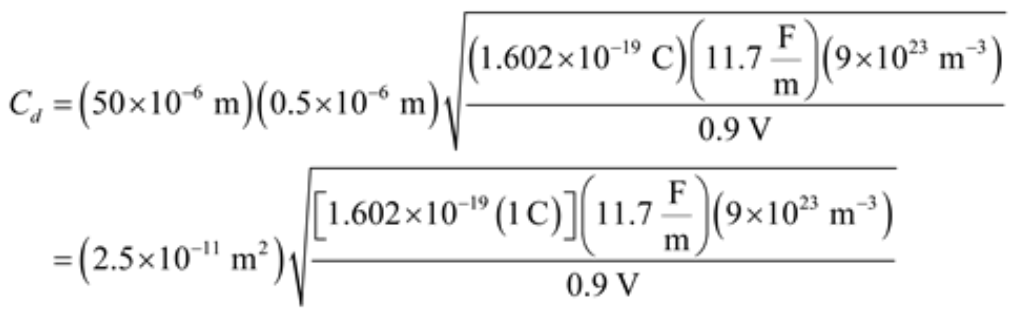
\includegraphics{2.15-21}
	\end{minipage}
\end{figure}

\begin{figure}[H] %H为当前位置,!htb为忽略美学标准,htbp为浮动图形
	\begin{minipage}{\linewidth}
		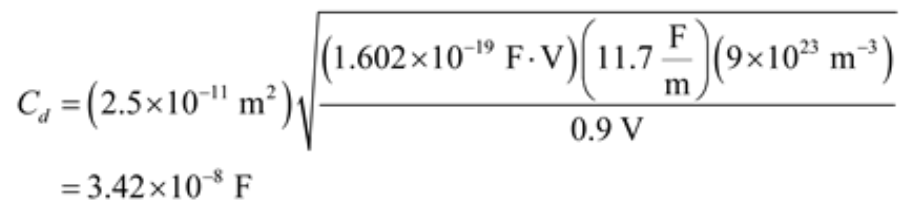
\includegraphics{2.15-22}
	\end{minipage}
\end{figure}

\begin{figure}[H] %H为当前位置,!htb为忽略美学标准,htbp为浮动图形
	\begin{minipage}{\linewidth}
		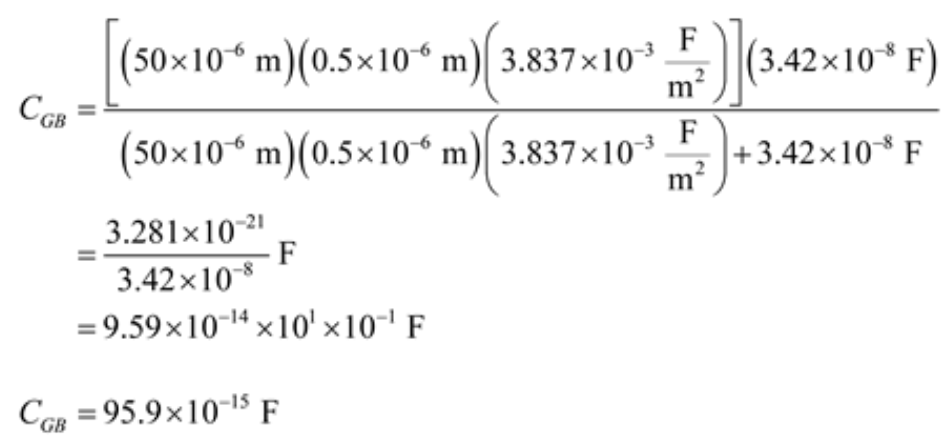
\includegraphics{2.15-23}
	\end{minipage}
\end{figure}








$C_{GB}=95.9fF$


$g_m=\frac{2I_D}{V_{GS}-V_{TH}}$\textcolor{blue}{(P18的2.20)}

\begin{figure}[H] %H为当前位置,!htb为忽略美学标准,htbp为浮动图形
	\begin{minipage}{\linewidth}
		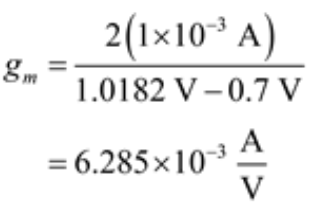
\includegraphics{2.15-24}
	\end{minipage}
\end{figure}







\begin{figure}[H] %H为当前位置,!htb为忽略美学标准,htbp为浮动图形
	\begin{minipage}{\linewidth}
		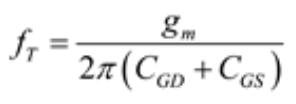
\includegraphics{2.15-25}
	\end{minipage}
\end{figure}

\begin{figure}[H] %H为当前位置,!htb为忽略美学标准,htbp为浮动图形
	\begin{minipage}{\linewidth}
		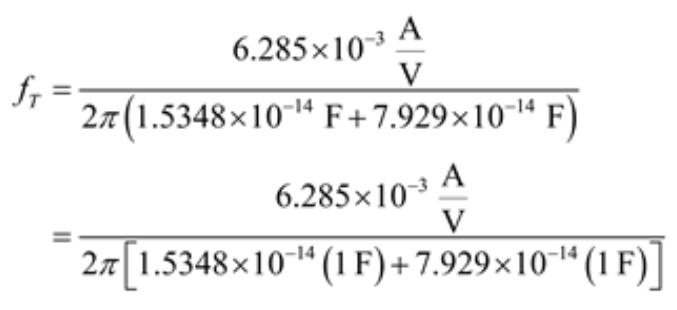
\includegraphics{2.15-26}
	\end{minipage}
\end{figure}

\begin{figure}[H] %H为当前位置,!htb为忽略美学标准,htbp为浮动图形
	\begin{minipage}{\linewidth}
		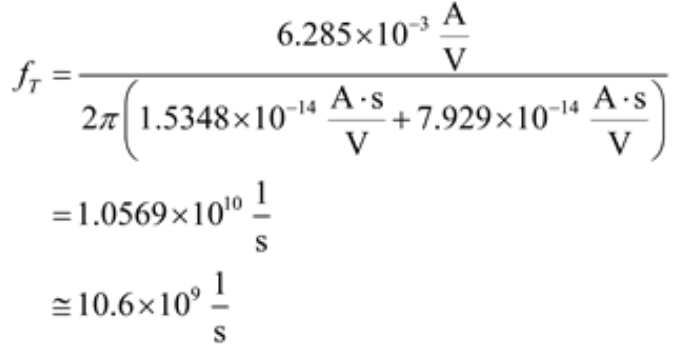
\includegraphics{2.15-27}
	\end{minipage}
\end{figure}


把上式的$\frac{1}{s}$换为$Hz$

$f_T=10.6 \times 10^9Hz$

$1G=10^9$

$f_T=10.6GHz$




	\color{green}{
	\{
	
	$C_j$和$C_{jsw}$公式和$C_d$
	
	
	
	
	
	
	
	
	\}
	
	
	
	
	
	
}









\color{black}{}